En este capítulo se analizará el uso de la plantilla. Además de los elementos propios de la plantilla se presentarán los elementos básicos de \LaTeX.

\section{Plantilla}

La plantilla consta de varios ficheros. El fichero principal es \texttt{main.tex}. Además, hay otros ficheros en la carpeta \texttt{config}. En principio no es necesario tocar estos ficheros.

En el fichero principal hay varias cosas que se pueden configurar.

Lo primero, la plantilla se basa en el estilo \texttt{memoir}. Por tanto, es posible usar todas las opciones asociadas a dicho estilo. Principalmente, se puede cambiar el estilo de los capítulos. Para ello, en el fichero \texttt{main.tex} al comienzo hay un comando, \texttt{chapterstyle}, con el que se puede definir el estilo. Estas son las opciones disponibles.
\begin{itemize}
	\item bianchi
	\item bringhurst
	\item brotherton
	\item chappell
	\item crosshead
	\item culver
	\item dash
	\item demo2
	\item demo3
	\item dowding
	\item \textbf{ell}
	\item ger
	\item komalike
	\item lyhne
	\item madsen
	\item ntglike
	\item pedersen
	\item \textbf{southall}
	\item \textbf{tandh}
	\item thatcher
	\item veelo
	\item \textbf{verville}
	\item \textbf{wilsondob}
\end{itemize}

Las opciones marcadas en negrita no incluyen el término ``capítulo'', por lo que son apropiadas para memorias en Euskara (en las figuras el orden del termino y el número están cambiados, pero no en los capítulos).

\subsection{Información sobre el proyecto}

Una vez definido el estilo encontramos los comandos para definir la información general del trabajo: autor/a, título, director/a/es/as y fecha del documento.

A continuación aparece la información relativa a la titulación. Para ello hay que definir dos comandos, \texttt{ikasketak} y \texttt{espezialitatea}, descomentando las opciones adecuadas y comentando el resto. El comando de la especialidad solo es necesario para el Grado en Ingeniería Informática.

\subsection{Idioma del documento}

El documento puede estar en castellano, euskara o inglés. Para configurar adecuadamente todos los cambios necesarios, en el fichero \texttt{main.tex} se puede definir el idioma descomentando la opción adecuada y comentando el resto. Solo una de las opciones debe estar descomentada.

\begin{table}[t]
	\centering
	\begin{tabular}{l|llll}
		Y  & A  & B  & C  & D  \\
		\hline
		y1 & a1 & b1 & c1 & d1 \\
		y2 & a2 & b2 & c2 & d2 \\
	\end{tabular}
	\caption {Ejemplo de tabla}\label{tab:ejemplo}
\end{table}

\subsection{Portada del documento}

Hay dos opciones para la portada. La primera es incrustar un PDF. Por defecto se incluye el documento \texttt{cover.pdf}. En caso de querer desactivar esta opción hay que comentar la línea que contiene el comando \texttt{includepdf}.

La segunda opción es usar los ficheors \texttt{cover\_XXX}. Hay tres, uno para el Grado en Ingeniería Informática, otro para el Grado en Inteligencia Artificial y otro para Trabajos Fin de Máster. Hay que descomentar el que interese y mantener comentados el resto.

Se puede usar una de las dos opciones o ambas, pero en cualquier caso es necesario que apareza la información contenida en los ficheros \texttt{cover\_XXX}. Si el PDF no incluye esta información, será necesario incluir ambas portadas.


\subsection{Contenido del documento}

A fin de facilitar la organización del texto el contenido está dividido en ficheros por capítulos en la carpeta \texttt{chapters}. A pesar del que el código está en dichos ficheros, a fin de tener una idea clara de la organización el título de los capítulos se define en el fichero \texttt{main.tex}.


\section{Figuras y tablas}

\begin{figure}[t]
	\centering
	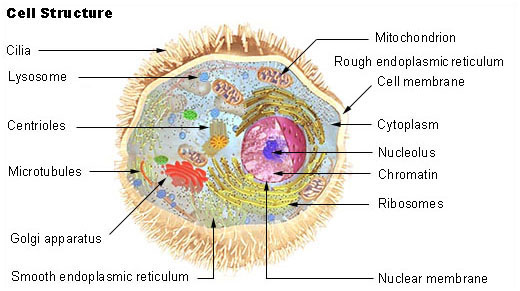
\includegraphics[width=0.75\textwidth]{figures/cell.jpg}
	\caption{Irudiaren adibidea}\label{fig:ejemplo}
\end{figure}

Con el objetivo de mantener el aspecto del documento se recomienda que las figuras y tablas estén todas arriba o abajo. Para ello es necesario usar las opciones \texttt{[t]} o \texttt{[b]} en los entornos \texttt{figure} y \texttt{table}.

La Figura \ref{fig:ejemplo} y la Tabla \ref{tab:ejemplo} muestran dos ejemplos. Hay que tener en cuenta que \LaTeX trata de optimizar la localización de la figuras y tablas. Como se ha mencionado, es recomendable seguir un criterio fijo (todas arriba o todas abajo). Para cambiar la hoja en la que aparece una figura o tabla hay que mover de lugar su código. Dicho código no tiene por que estar donde se menciona en el texto, ya que la referencia a las figuras y tablas debe hacerse usando su número y no usando términos como ``abajo'' o ``arriba''.

\section{Elementos matemáticos}

Muchos de los elementos se definen en el paquete \texttt{ifcommands}. En el fichero \texttt{main.tex} al comienzo se carga dicho paquete y ahí se puede escoger el idioma deseado.

A continuación se muestran los elementos definidos en el paquete.

\begin{ifaxiom}
	Ejemplo de axioma
\end{ifaxiom}

\begin{iftheorem}
	Ejemplo de teorema
\end{iftheorem}

\begin{iflemma}
	Ejemplo de lema
\end{iflemma}

\begin{ifproposition}
	Ejemplo de proposición
\end{ifproposition}

\begin{ifdefinition}
	Ejemplo de definición
\end{ifdefinition}

\begin{ifexample}
	Ejemplo de ejemplo
\end{ifexample}

\begin{ifproblem}
	Ejemplo de problema
\end{ifproblem}

\begin{ifsolution}
	Ejemplo de solución
\end{ifsolution}

\begin{ifremark}
	Ejemplo de comentario
\end{ifremark}

\begin{ifalgorithm}[t]
	\begin{ifpseudo}{Nombre del algoritmo}
		\item	\In\ Sarrera
		\item	\Out\ Irteera
		\item	\For{1}{n}
		\item	\T{Lehenengo urratsa}
		\item	\EFor
		\item	\If\ baldintza \Then
		\item	\T{\While{beste baldintza}}
		\item	\TT{errepikatzeko urratsa}
		\item	\T{\Done}
		\item	\Else
		\item	\T{\Do}
		\item	\TT{\CFor elementu bakoitza}
		\item	\TTT{elementua prozesatu}
		\item	\TT{\EFor}
		\item	\T{\Until{hirugarren baldintza}}
		\item	\EIf
		\item	\WhileDo{azken baldintza}
		\item	\T{\If amaitu}
		\item	\TT{\Return}
		\item	\T{\EIf}
	\end{ifpseudo}
	\caption{Ejemplo de pseudocódigo}\label{alg:ejemplo}
\end{ifalgorithm}

Además de estos elementos existen dos entornos para definir algoritmos, \texttt{ifalgorithm} y \texttt{ifpseudo}. También es posible incluir un índice de algoritmos además de los índices de tablas y figuras. En el Algoritmo \ref{alg:ejemplo} se muestra un ejemplo de la sintaxis.

Por último, en lo que respecta a las ecuaciones matemáticas, estas pueden estar en el texto: $X_n \geq 10$, o intercaladas con el:

\begin{eqnarray}
	P(\Theta|D) = \frac{P(D|\Theta)P(\Theta)}{P(D)}\\
	P(\Theta) \sim Beta(\alpha, \beta)
\end{eqnarray}

También se pueden incluir ecuaciones sin numeración:

\begin{eqnarray*}
	P(\Theta|D) = \frac{P(D|\Theta)P(\Theta)}{P(D)}\\
	P(\Theta) \sim Beta(\alpha, \beta)
\end{eqnarray*}



\section{Referencias}

Para añadir la bibliografía hay que usar BibTeX. Las referencias están recogidas en el fichero \texttt{erreferentziak.bib} y en el texto se citan usando el comando \texttt{cite}. Por ejemplo, \cite{Shahbaba2011} o \cite{Efron1994, Rmanual, Subramanian2005gene}. No hay que olvidar añadir toda la información de las referencias (páginas, año, etc.).